\section{Deployment view}

This section shows the configuration of the runtime processing nodes and the components that live on them. In the \textbf{figure \ref{fig:Deployment}} there is a representation of the Deployment diagram for the entire system.
The firewalls and DMZ are omitted in the diagram for readability, but they are treated in the Overview section.

In the package \emph{Client} there are five nodes, one for each client app; since the apps are multiplatform the nodes can either be on iOS or Android and all of them communicate with the \emph{Web Server} node through the TCP/IP protocol. 
Client nodes can be:
\begin{enumerate}
    \item \textbf{D4HIndividual} (it is the only client that communicates with a \emph{Smartwatch or Fitness band} through a Bluetooth connection)
    \item \textbf{D4HThird-party}
    \item \textbf{ASOSUser}
    \item \textbf{T4RRunner}
    \item \textbf{T4ROrganizer}
\end{enumerate}

In the \emph{Server} package there are four different physical nodes; three of them are one per application: D4H, ASOS and T4R. A main role is played by the fourth node: the \textbf{Web Server}. The \emph{Web Server} interfaces, on the front-end, with client applications and, on the back-end, with application servers. It provides the clients with the required informations queried from a specific application server and encapsulated in a structured format such as JSON or XML; by masking the presence of back-end servers it provides an effective security measure.
The \emph{Web Server} and the three application nodes communicate between each other through the TCP/IP protocol.

The \emph{Database Server} package contains two physical databases; one is dedicated to the Data4Help system, the other one stores Track4Run data. Only D4H has the access to the D4H database and only T4R has the access to the T4R database. Both of them comunicate with their databases through the TCP/IP protocol.

The two remaining nodes represent external services that apps make use of, in order to reach their goals:
\begin{itemize}
    \item \textbf{Ambulance service}: it communicates only with the ASOS nodes, through TCP/IP protocol. 
    \item \textbf{Google Maps service}: It is connected with D4H and T4R nodes through TCP/IP protocol.
\end{itemize}

\begin{figure}[htbp]
    \centering
    \makebox[\textwidth][c]{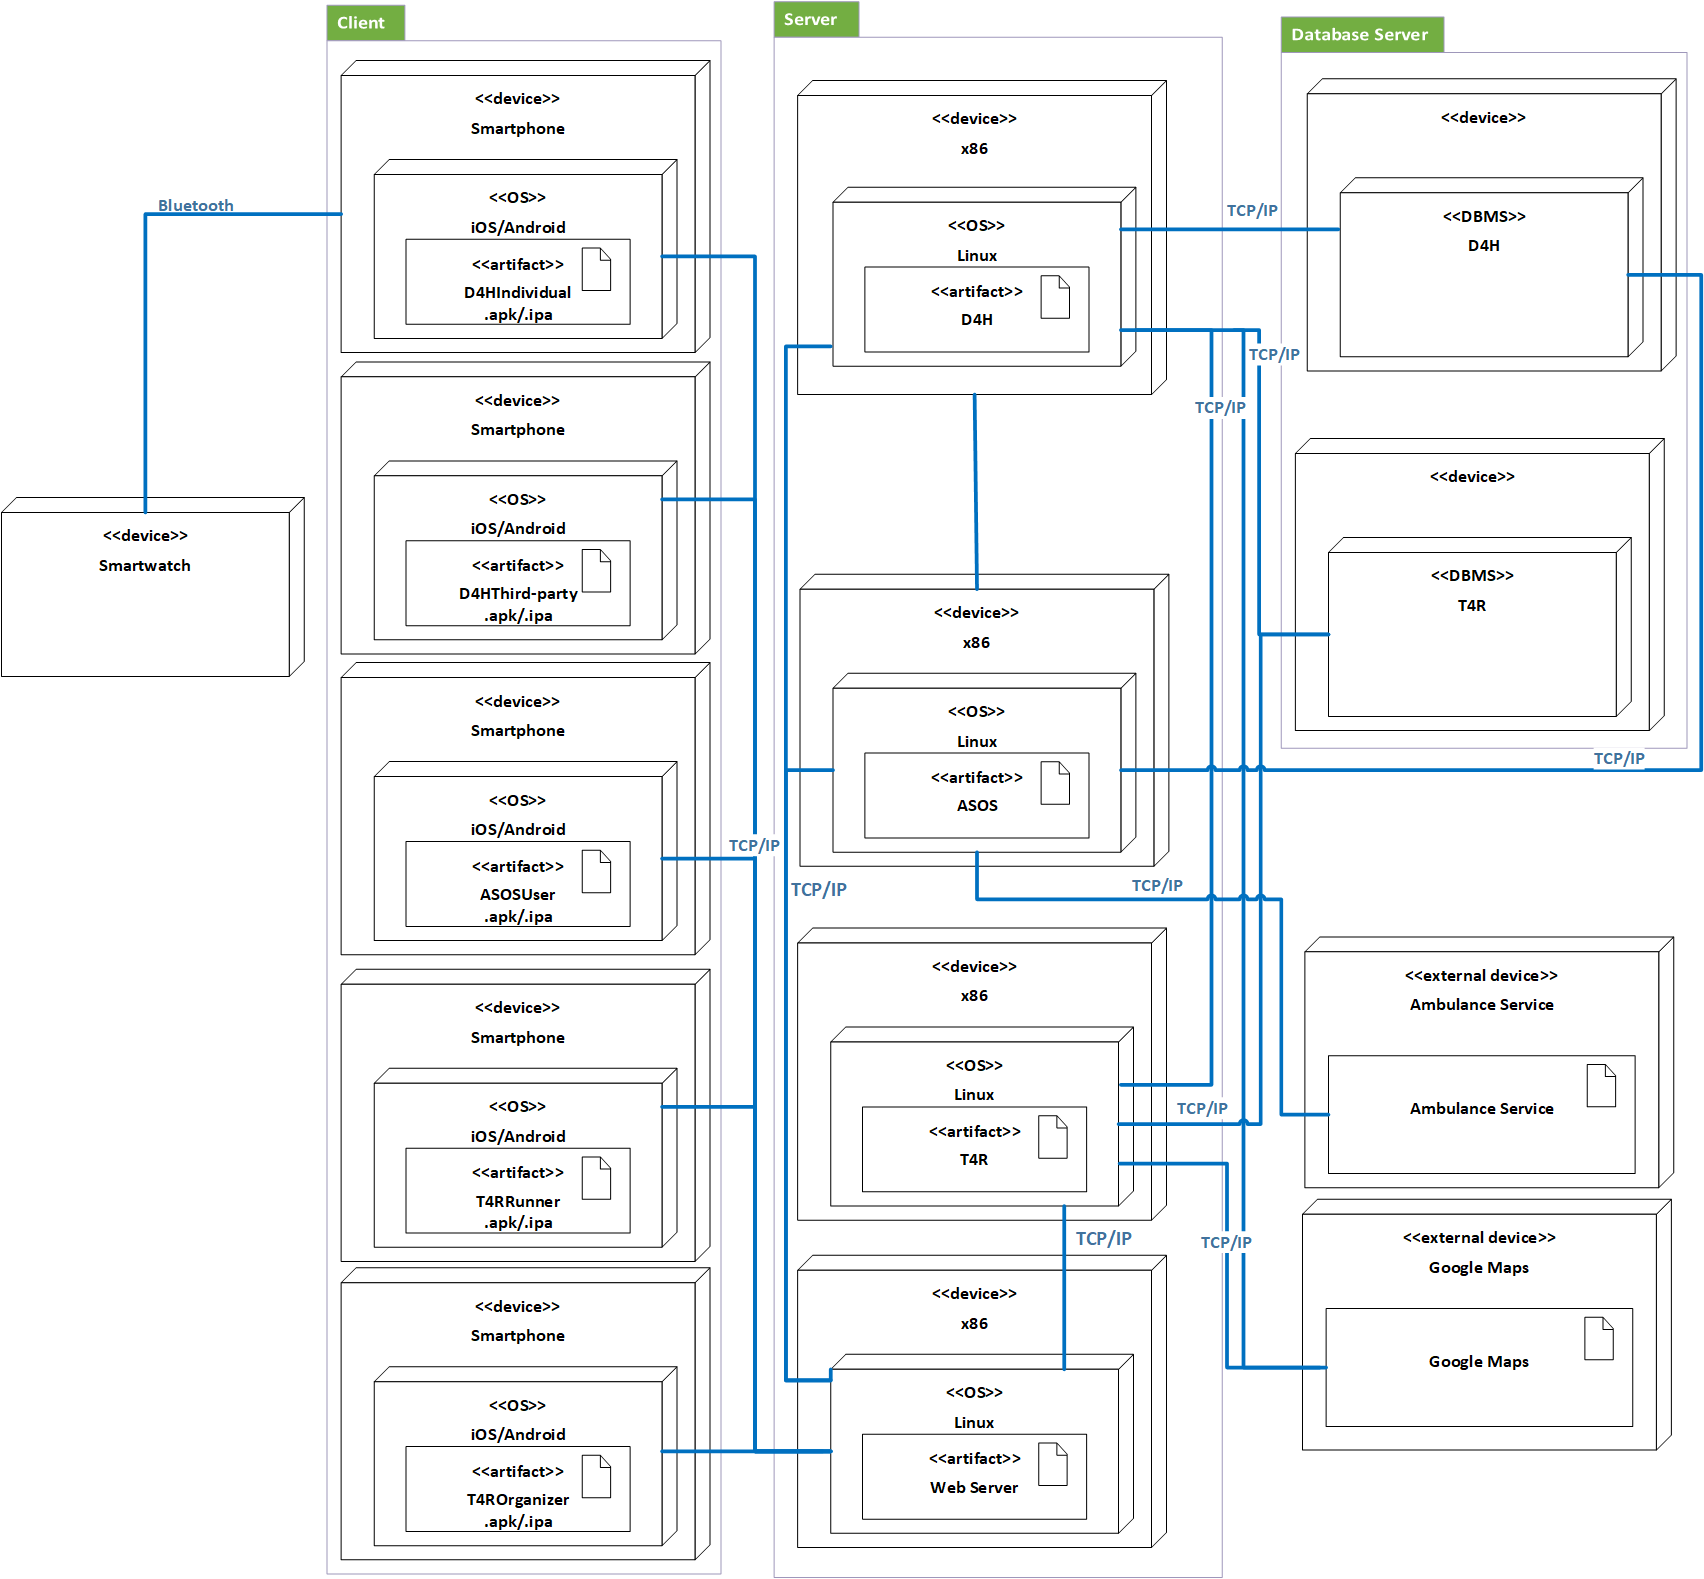
\includegraphics[scale=0.50]{pictures/deploymentDiagram.png}}
    \caption{Deployment Diagram for the entire system}
    \label{fig:Deployment}
\end{figure}